\section{Method}
\label{sec:method}

\begin{figure}[t]
\centering
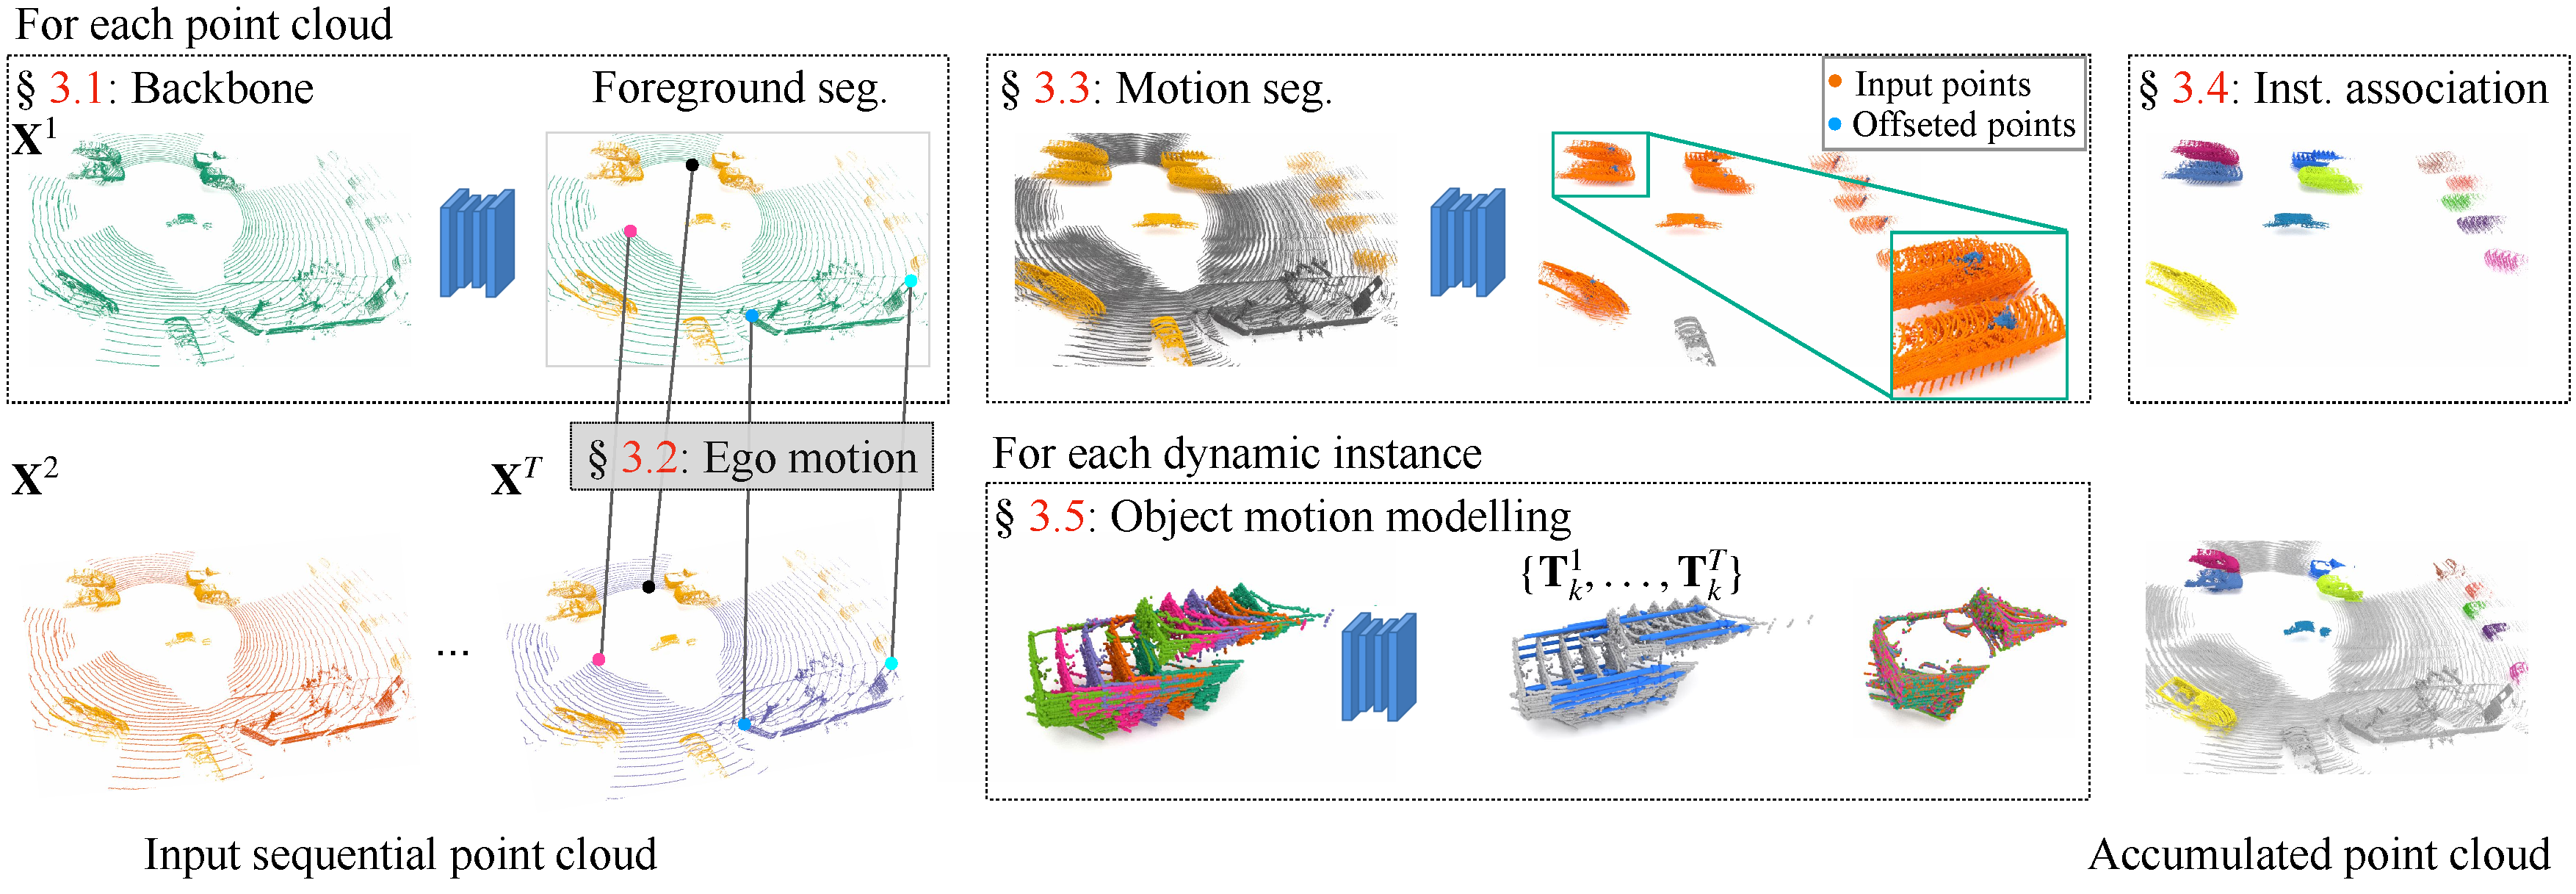
\includegraphics[width=1.0\textwidth]{content/main/images/overview.pdf}
\caption{Left: real LiDAR scan demonstrating key LiDAR return properties: a \textcolor{mygray}{single return} and two returns (first return shown in \textcolor{myblue}{blue} and second return in \textcolor{myorange}{orange}). Right: NFL models the waveform and accurately reproduces these properties. (a) Top: the LiDAR energy is fully scattered by the first surface. Bottom: NFL estimates range via peak detection on the computed weights $w$ followed by volume rendering based range refinement. (b) Top: secondary returns resulting from a beam hitting two surfaces. Bottom: NFL employs beam divergence and a truncated volume rendering to estimate the second return. (c) Top: beams that do not hit a surface do not return detectable signal. Bottom: NFL utilizes geometric and semantic features to predict the ray drop probability. Refer to section \ref{sec:render_lidar} for more details. }
\label{fig:overview}
\end{figure}


The network architecture of our multitask model is schematically depicted in \cref{fig:architecture}. To accumulate the points over time, we make use of the inductive bias that scenes can be decomposed into agents that move as rigid bodies~\cite{gojcic2021weakly}. We start by extracting the latent base features of each individual frame~(\cref{sec:backbone_network}), which we then use as input to the task-specific heads. To estimate the ego-motion, we employ a differentiable registration module (\cref{sec:ego_motion}). Instead of using the ego-motion only to align the static scene parts, we also use it to spatially align the base features, which are reused in the later stages. To explain the motion of the dynamic foreground, we utilize the aligned base features and perform motion segmentation (\cref{sec:motion_seg}) as well as spatio-temporal association of dynamic foreground objects (\cref{sec:clustering}). Finally, we decode the rigid body motion of each foreground object from its spatio-temporal features (\cref{sec:dynamic_obj}). We train the entire model end-to-end with a loss $\loss$ composed of five terms: 
\begin{equation}
    \loss = \loss_\ego^\lcircle{lossred} + \loss_\FG^\lcircle{lossgreen} + \loss_\motion^\lcircle{lossblue} + \lambda_\textoffset\loss_\textoffset^\lcircle{lossyellow} + \lambda_{\text{obj}}\loss_{\text{obj}}^\lcircle{losspurple}\;.
    \label{eq:eccv_loss}
\end{equation}

\begin{equation}
    \loss = \loss_\ego + \loss_\FG + \loss_\motion + \lambda_\textoffset\loss_\textoffset + \lambda_{\text{obj}}\loss_{\text{obj}}\;.
\end{equation}

In the following, we provide a high-level description of each module. 
Detailed network architectures, including parameters and loss formulations, are given in the appendix (unless already elaborated).

\paragraph{Problem setting}
Consider an \textit{ordered} point cloud sequence $\PCset = \{\PC^t\}_{t=1}^T$ consisting of $T$ frames $\PC^t = [\point_1^t,...,\point_i^t,...,\point_{n_t}^t] \in \mathbb{R}^{3 \times n_t}$ of variable size, captured by a \textit{single moving observer} at constant time intervals $\Delta t$. We denote the first frame $\PC^1$ the \textit{target} frame, while the remaining frames $\{ \PC^{t} \; | \; t>1 \}$ are termed \textit{source} frames. Our goal is then to estimate the flow vectors $\{ \Flow^t \in \mathbb{R}^{3 \times n_t} | t>1 \}$ that align each of the source frames to the target frame, and hence \emph{accumulate} the point clouds. Instead of predicting unconstrained pointwise flow vectors, we make use of the inductive bias that each frame can be decomposed into a %
\textit{static} part $\PC^t_\static$ and $K_{t}$ rigidly-moving \textit{dynamic} parts $\PCset^t_{\text{dynamic}} = \{\PC^t_k\}_{k=1}^{K_t}$~\cite{gojcic2021weakly}. 
For an individual frame, the scene flow vectors $\Flow_\static^t$ of the static part and $\Flow_k^t$ of the $k$-th dynamic object can be explained by the rigid %
ego-motion
$\T_\ego^t \in \SEuc$ and the motion of the dynamic object relative to the static background $\T_k^t \in \SEuc$, respectively as:
\begin{equation}
\label{eq:sf}
    \Flow_\static^t = \T_\ego^t \circ \PC_\static^t - \PC_\static^t, \qquad
    \Flow_k^t = \T_k^t \T_\ego^t \circ \PC_k^t - \PC_k^t,
\end{equation}
where $\T\circ\PC$ (or $\T \circ \point$) denotes applying the transformation to the point set $\PC$ (or point $\point$).

\subsection{Backbone network}
\label{sec:backbone_network}
Similar to~\cite{baur2021slim,jund2021scalable,wu2020motionnet}, our backbone network converts the 3D point cloud of a single frame into a bird's eye view (BEV) 
latent feature image. Specifically, we lift the point coordinates to a higher-dimensional latent space using a point-wise MLP and then scatter them into a $H\times W$ feature grid aligned with the gravity axis. The features per grid cell (``pillar'') are aggregated with max-pooling, then fed through a 2D UNet~\cite{long2015fully} to enlarge their receptive field and strengthen the local context. The output of the backbone network is a 2D latent \emph{base} feature map $\Feature_\bev^t$ for each of the $T$ frames.

% \paragraph{Discussion on point cloud representation}
% An alternative to the BEV projection is sparse voxel~\cite{choy2019Minkowski}. We choose BEV for several reasons: \textit{(i)}. BEV is more efficient in both time and memory, allowing for potential online deployment; \textit{(ii)} BEV allows one to warp, stack, and reuse feature maps in a differentiable manner. Doing the same for sparse voxels is non-trivial; \textit{(iii)} compared to \cite{gojcic2021weakly} that uses a sparse voxel backbone, BEV turns out be to more robust to point density and thus improving the scene flow estimation (see \cref{sec:results}). 

\subsection{Ego-motion estimation}
\label{sec:ego_motion}
We estimate the ego-motion $\T_\ego^t$ using a correspondence-based registration module separately for each source frame. Points belonging to dynamic objects can bias the estimate of ego-motion, especially when using a correspondence-based approach, and should therefore be discarded. 
However, at an early stage of the pipeline it is challenging to reason about scene dynamics, so we rather follow the conservative approach and classify points into background and foreground, where foreground contains all the \emph{movable} objects (\eg, cars and pedestrians), irrespective of their actual dynamics~\cite{gojcic2021weakly}. 
The predicted foreground mask is later used to guide motion segmentation in \cref{sec:motion_seg}.

We start by extracting ego-motion features $\Feature^t_\geo$ and foreground scores $\s^t_\FG$ from each $\Feature_\bev^t$ using two dedicated heads, each consisting of two convolutional layers separated by a ReLU activation and batch normalization. We then randomly sample $N_\ego$ background pillars whose $\s^t_\FG < \tau$ and compute the pillar centroid coordinates $\mathbf{P}^t = \{\pillar_l^t \}$. The ego motion $\T^t_\ego$ is estimated as:
\begin{equation}
{\T^t_\ego} = \argmin_{\T} \sum_{l=1}^{N_\ego} w_l^t \left\|\T \circ \pillar_l^t - \phi(\pillar_l^t, \mathbf{P}^1)\right\|^2. 
\label{eq: ego-motion}
\end{equation}
%
Here, $\phi(\pillar_l^t, \mathbf{P}^1)$ finds the \emph{soft correspondence} of $\mathbf{p}_l^t$ in $\mathbf{P}^1$, and $w_l^t$ is the weight of the correspondence pair $\big(\pillar_l^t, \phi(\pillar_l^t, \mathbf{P}^1)\big)$. Both $\phi(\pillar_l^t, \mathbf{P}^1)$ and $w_l^t$ are estimated using an entropy-regularized Sinkhorn algorithm from $\Feature_\geo^t$ with slack row/column padded~\cite{cuturi2013sinkhorn,yew2020rpm} and the optimal $\T^t_\ego$ is computed in closed form via the differentiable Kabsch algorithm~\cite{kabsch1976solution}.

We supervise the ego-motion with an $L_1$ loss over the transformed pillars $\loss_\trans =\frac{1}{|\mathbf{P}^t|}  \sum_{l=1}^{|\mathbf{P}^t|} \| \T \circ \pillar_l^t - \overline{\T} \circ \pillar_l^t \|_{1}$ and an inlier loss $\loss_{\text{inlier}}$~\cite{yew2020rpm} that regularizes the Sinkhorn algorithm, $\loss_\ego^\lcircle{lossred}=\loss_\trans + \loss_{\text{inlier}}$.
The foreground score $\s_\FG^t$ is supervised using a combination of weighted binary cross-entropy (BCE) loss $\loss_{\text{bce}}$ and Lovasz-Softmax loss $\loss_{\text{ls}}$~\cite{berman2018lovasz}: $\loss_\FG^\lcircle{lossgreen} = \loss_{\text{bce}}(\s_\FG^t, \overline{\s}_\FG^t) + \loss_{\text{ls}}(\s_\FG^t, \overline{\s}_\FG^t)$, with $\overline{\s}^t_\FG$ the binary ground truth.
The weights in $\loss_{\text{bce}}$ are inversely proportional to the square root of elements in each class. 


\subsection{Motion segmentation}
\label{sec:motion_seg}
To separate the \emph{moving} objects from the \emph{static} ones we perform motion segmentation, reusing the per-frame base features $\{\Feature_\bev^t\}$.
Specifically, we apply a differentiable feature warping scheme~\cite{sun2018pwc} that warps each $\Feature_\bev^t$ using the predicted ego-motion $\T^t_\ego$, and obtain a spatio-temporal 3D feature tensor of size {\small${C\times T\times H\times W}$} by stacking the warped feature maps along the channel dimension.
This feature tensor is then fed through a series of 3D convolutional layers, followed by max-pooling across the temporal dimension $T$. 
Finally, we apply a small 2D UNet to obtain the 2D motion feature map $\Feature_\motion$.

To mitigate discretization error, we bilinearly interpolate grid motion features to all foreground points in each frame.\footnote{We predict motion labels only for foreground and treat background points as static.}
The point-level motion feature for $\point_i^t$ is computed as:
\begin{equation}
    \label{eq:point-motion}
    \feature_{\motion,i}^t =\MLP\big(\cat[\psi(\point_i^t,\Feature_\motion), \MLP(\point_i^t)]\big),
\end{equation}
where $\MLP(\cdot)$ denotes a multi-layer perceptron, $\cat[\cdot]$ concatenation, and $\psi(\point, \Feature)$ a bilinear interpolation from $\Feature$ to $\point$.
The dynamic score $\s_i^t$ of the point $\point_i^t$ is then decoded from the motion feature $\feature_{\motion,i}^t$ using another MLP, and supervised similar to the foreground segmentation, with a loss $\loss_\motion^\lcircle{lossblue} = \loss_{\text{bce}}(\s_i^t, \overline{\s}_i^t) + \loss_{\text{ls}}(\s_i^t, \overline{\s}_i^t)$, where $\overline{\s}_i^t$ denotes the ground-truth motion label of point $\point_i^t$.

\subsection{Spatio-temporal instance association}
\label{sec:clustering}
To segment the dynamic points (extracted by thresholding the $\s_i^t$) into individual objects and associate them over time, we perform spatio-temporal instance association.
Different from the common tracking-by-detection~\cite{dendorfer2021motchallenge,weng20203d} paradigm, we propose to directly \emph{cluster the spatio-temporal point cloud}, which simultaneously provides instance masks and the corresponding associations.
However, naive clustering of the ego-motion aligned point clouds often fails due to LiDAR sparsity and fast object motions, hence we predict a per-point offset vector $\offset_i^t$ pointing towards %
the (motion-compensated) instance center:
\begin{equation}
    \offset_{i}^t = \MLP\big(\cat[\psi(\point_i^t, \Feature_\motion), \MLP(\point_i^t)]\big).
\end{equation}

The DBSCAN~\cite{ester1996density} algorithm is subsequently applied over the deformed point set $\{\point_i^t + \offset_i^t \; | \; \forall i, \forall t\}$ to obtain an instance index for each point.
This association scheme is simple yet robust, and can seamlessly handle occlusions and mis-detections.
Similar to 3DIS~\cite{lahoud20193d} we supervise the offset predictions $\offset_i^t$ with both an $L_1$-distance loss and a directional
loss:
\begin{equation}
\loss_\textoffset^\lcircle{lossyellow} =\frac{1}{n}  \sum_{\{i,t\}}^n \left( \left\| \offset_i^t  - \overline{\offset}_i^t \right\|_{1} + 1 - \langle \frac{\offset_i^t}{\| \offset_i^t\|}, \frac{\overline{\offset}_i^t}{\| \overline{\offset}_i^t\|} \rangle \right),
\end{equation}
where $\overline{\offset}$ is the ground truth offset $\mathbf{o}-\point$ from the associated instance centroid $\mathbf{o}$ in the target frame, and $\langle \cdot \rangle$ is the inner product.


\subsection{Dynamic object motion modelling}
\label{sec:dynamic_obj}
Once we have spatio-temporally segmented objects, we must
recover their motions at each frame.
As LiDAR points belonging to a single object are sparse and explicit inter-frame correspondences are hard to find, we take a different approach from the one used in the ego-motion head and construct a novel TubeNet to directly regress the transformations.
Specifically, TubeNet takes $T$ frames of the same instance $\mathbf{X}_k$ as input, and regresses its rigid motion parameters $\T^t_k$ as:
\begin{equation}
    \T^t_k = \MLP \left(\cat[ \agfeature_{\motion}, \agfeature_\ego, \agfeature_{\pos}^t, \agfeature_{\pos}^1] \right),
    \label{eq:tubenet}
\end{equation}
where $\agfeature_\motion$ and $\agfeature_\ego$ are instance-level global features obtained by applying PointNet~\cite{qi2017pointnet} to the respective point-level features of that instance, $\agfeature_{\type} = \PN(\{ \feature_{\type,i}^t \; | \; \point_i^t \in \PC_k^t \})$.
Recall that point-level features $\feature_{\type,i}^t$ are computed from $\Feature_{\type}$ via the interpolation scheme described in \cref{eq:point-motion}.
Here, $\agfeature_\motion$ encodes the overall instance motion while $\agfeature_\ego$ supplements additional geometric cues. The feature
$\agfeature_\pos^t = \PN(\PC_k^t)$ is a summarized encoding over individual frames and provides direct positional information for accurate transformation estimation. 
%
The transformations are initialised to identity and TubeNet is applied in iterative fashion to regress residual transformations relative to the last iteration, similar to RPMNet~\cite{yew2020rpm}.

For the loss function, we choose to parameterise each $\T$ as an un-normalised quaternion $\quat \in \real^{4}$ and translation vector $\tvec \in \real^3$, and supervise it with:
\begin{equation}
    \loss_\obj^\lcircle{losspurple} = \loss_\trans + \frac{1}{T-1} \sum_{t=2}^T \left( \left\|\overline{\tvec}_k^t - \tvec_k^t \right\|_2 + \lambda \left\|\overline{\quat}_k^t - \frac{\quat_k^t}{{\|\quat_k^t}\|} \right\|_2 \right),
\end{equation}
where $\overline{\tvec}_k^t$ and $\overline{\quat}_k^t$ are the ground truth transformation, and $\lambda$ is a constant weight, set to 50 in our experiments. 
$\loss_\trans$ is the same as in the ego-motion (\cref{sec:ego_motion}).


\subsection{Comparison to related work}
\paragraph{WsRSF~\cite{gojcic2021weakly}} Our proposed method differs from WsRSF in several ways: \textit{(i)} WsRSF is a pair-wise scene flow estimation method, while we can handle multiple frames; \textit{(ii)} unlike WsRSF we perform motion segmentation for a more complete understanding of the scene dynamics; \textit{(iii)} our method outputs instance-level associations, while WsRSF simply connects each instance to the complete foreground of the other point cloud.

\paragraph{MotionNet~\cite{wu2020motionnet}} Similar to our method, MotionNet also deals with sequential point clouds and uses a BEV representation. However, MotionNet \textit{(i)} assumes that ground truth ego-motion is available, while we estimate it within our network; and \textit{(ii)} does not provide object-level understanding, rather it only separates the scene into a static and a dynamic part. 

\subsection{Implementation details}
Our model is implemented in pytorch~\cite{NEURIPS2019_9015} and can be trained on a single RTX 3090 GPU. During training we minimize \cref{eq:eccv_loss} with the Adam~\cite{kingma2014adam} optimiser, with an initial learning rate 0.0005 that exponentially decays at a rate of 0.98 per epoch. For both \emph{Waymo} and \emph{nuScenes}, the size of the pillars is $(\delta_x, \delta_y, \delta_z) = (0.25, 0.25, 8)$ m. We sample $N_{\text{ego}} = 1024$ points for ego-motion estimation and set $\tau =0.5$ for foreground/background segmentation. The feature dimensions of $\Feature_\bev^t$, $\Feature_\ego^t$, $\Feature_\motion$ are 32, 64, 64 respectively. During inference we additionally use ICP~\cite{besl1992method} to perform test-time optimisation of the ego-motion as well as the transformation parameters of each dynamic object. ICP thresholds for ego-motion and dynamic object motion are 0.1/0.2 and 0.15/0.25 $\,$m for \emph{Waymo} / \emph{nuScenes}. 




